The SWinIR model proposed by Liang et al. \cite{liangSwinIRImageRestoration2021a}, 
makes use of the shifted window transfomer architecture introduced by Liu et al. \cite{liangSwinIRImageRestoration2021a}.
While the model does not employ the hierarchical structure of the original architecture, 
it makes extensive use of the shifted window mechanism.
The model architecture is depicted in figure \ref{fig:swinir_model}.

\begin{figure}[h!]
    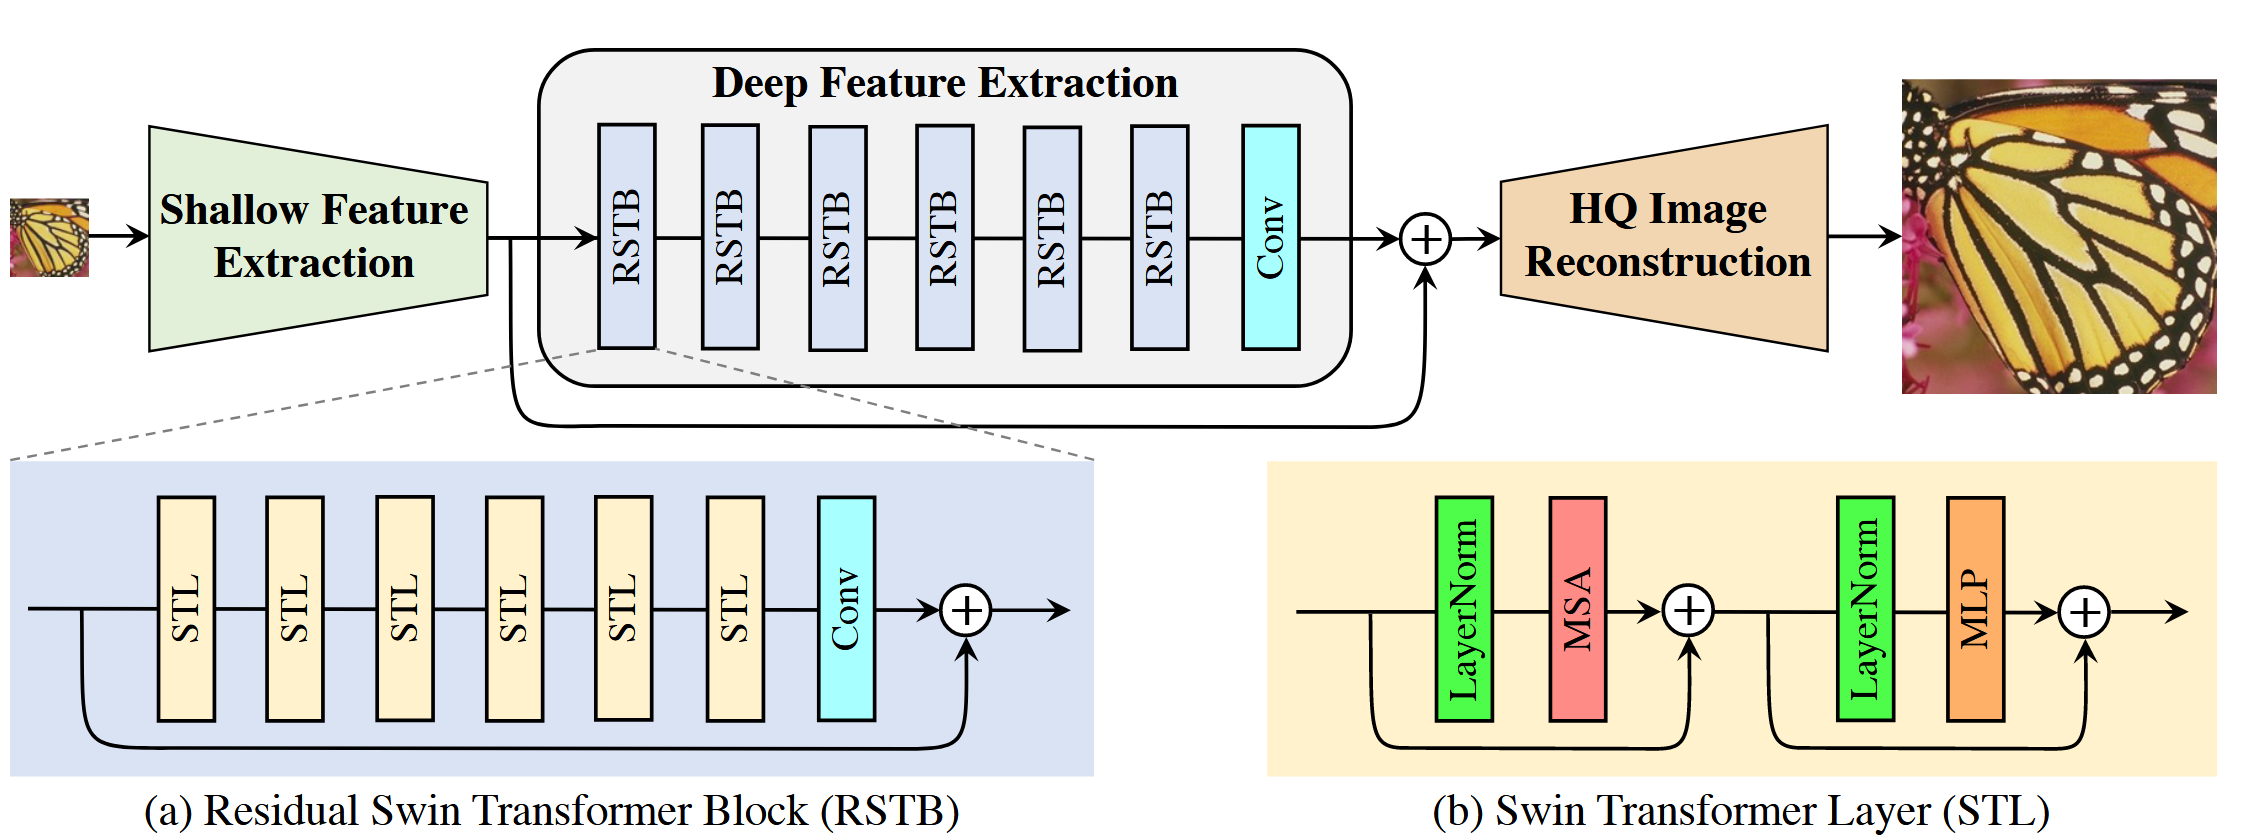
\includegraphics[width=0.9\textwidth]{models/sisr/imgs/swinir_model.png}
    \caption{Image taken from \cite{liangSwinIRImageRestoration2021a}, architecture of SWinIR model.}
    \label{fig:swinir_model}
\end{figure}

The broader architectural design follows that described in section \ref{sec:general_model}.
Given inputs $X \in \mathbb R^{3 \times H \times W}$, 
the shallow feature extraction is performed via a single convolutional layers

    $$F_0 = C(3, 180, \text{kernel-size}=3, \text{padding}=1)(X) ~.$$

The features are then further processed by the deep feature extraction module

    $$F_1 = H_D(F_0) + F_0 ~,$$

before being upsampled using the image reconstruction module $I_{SR} = H_{IR}(F_1)$.
To this end the authors employ a sub-pixel convolutional layer. \newline

The deep feature extraction module is composed of $6$ Residual Swin Transformer Blocks (RSTBs),
followed by a last convolutional layer

    $$H_D = C(180, 180) \circ H_{RSTB} \circ ... \circ H_{RSTB} ~.$$

Each RSTB is consists of $6$ Transformer layers where every second makes use of the shifted window mechanism, 
these are suceeded by a final convolutional layer

    $$H_{RSTB} = C(180, 180) \circ H_{STL} \circ H_{TL} \circ ... \circ \circ H_{STL} \circ H_{TL} ~.$$

